\section{Python integration}
\label{sec:python}
A recent feature of Mitsuba is a Python interface to the renderer API.
To use this interface, start your Python interpreter and simply enter
\begin{python}
import mitsuba
\end{python}
\paragraph{Mac OS:}
For this to work on MacOS X, you will first have to run the ``\emph{Apple
Menu}$\to$\emph{Command-line access}'' menu item from within Mitsuba.
If you compiled Mitsuba yourself, then an alternative way of setting the appropriate
environment variables without making changes to the system is by sourcing the
\code{setpath.sh} script located in the main Mitsuba directory.

\paragraph{Linux:}
If you installed one of the official Mitsuba packages for your distribution, then everything should work out of the box.
If you compiled Mitsuba yourself, you will need to source the
\code{setpath.sh} script located in the main Mitsuba directory before starting Python.

\paragraph{Windows}
On Windows it is necessary to explicitly specify the required extension search path within Python
before issuing the \code{import} command, e.g.:
\begin{python}
import os, sys

# NOTE: remember to specify paths using FORWARD slashes (i.e. '/' instead of
# '\' to avoid pitfalls with string escaping)

# Configure the search path for the Python extension module
sys.path.append('path-to-mitsuba-dist-directory/python/<python version, e.g. 2.7>')

# Ensure that Python will be able to find the Mitsuba core libraries
os.environ['PATH'] = 'path-to-mitsuba-dist-directory' + os.pathsep + os.environ['PATH']

import mitsuba
\end{python}
If you get an error message ``\code{ImportError: DLL load failed: \%1 is not a valid Win32 application}'',
    the Python and Mitsuba architectures are mismatched (\code{i386} vs \code{x86\_64}).

\subsubsection*{Python API documentation}
For an overview of the currently exposed API subset, please refer
to the following page: \url{http://www.mitsuba-renderer.org/api/group__libpython.html}.

The plugin also exports comprehensive Python-style docstrings, hence
the following is an alternative way of getting information on
classes, function, or entire namespaces within an interactive Python shell:
\begin{shell}
>>> help(mitsuba.core.Bitmap) # (can be applied to namespaces, classes, functions, etc.)

 class Bitmap(Object)
  |  Method resolution order:
  |      Bitmap
  |      Object
  |      Boost.Python.instance
  |      __builtin__.object
  |
  |  Methods defined here:
  |  __init__(...)
  |      __init__( (object)arg1, (EPixelFormat)arg2, (EComponentFormat)arg3, (Vector2i)arg4) -> None :
  |          C++ signature :
  |              void __init__(_object*,mitsuba::Bitmap::EPixelFormat,mitsuba::Bitmap::EComponentFormat,mitsuba::TVector2<int>)
  |
  |      __init__( (object)arg1, (EFileFormat)arg2, (Stream)arg3) -> None :
  |          C++ signature :
  |              void __init__(_object*,mitsuba::Bitmap::EFileFormat,mitsuba::Stream*)
  |
  |  clear(...)
  |      clear( (Bitmap)arg1) -> None :
  |          C++ signature :
  |              void clear(mitsuba::Bitmap {lvalue})
...
\end{shell}
The docstrings list the currently exported functionality, as well as C++ and Python signatures, but they
don't document what these functions actually do. The web API documentation is
the preferred source for this information.

\subsection{Basics}
Generally, the Python API tries to mimic the C++ API as closely as possible.
Where applicable, the Python classes and methods replicate overloaded operators,
virtual function calls (which can be overridden in Python), and default arguments. Under rare circumstances,
some features are inherently non-portable due to fundamental differences between the
two programming languages. In this case, the API documentation will contain further
information.

Mitsuba's linear algebra-related classes are usable with essentially the
same syntax as their C++ versions --- for example, the following snippet
creates and rotates a unit vector.
\begin{python}
import mitsuba
from mitsuba.core import *

# Create a normalized direction vector
myVector = normalize(Vector(1.0, 2.0, 3.0))

# 90 deg. rotation around the Y axis
trafo = Transform.rotate(Vector(0, 1, 0), 90)

# Apply the rotation and display the result
print(trafo * myVector)
\end{python}

\subsection{Recipes}
The following section contains a series of ``recipes'' on how to do
certain things with the help of the Python bindings.
To copy and paste from this chapter, the \LaTeX source code may
be more convenient. It is available at the following URL: \url{https://www.mitsuba-renderer.org/repos/mitsuba/files/tip/doc/python.tex}.

\subsubsection{Loading a scene}
The following script demonstrates how to use the
\code{FileResolver} and \code{SceneHandler} classes to
load a Mitsuba scene from an XML file:
\begin{python}
import mitsuba

from mitsuba.core import *
from mitsuba.render import SceneHandler

# Get a reference to the thread's file resolver
fileResolver = Thread.getThread().getFileResolver()

# Register any searchs path needed to load scene resources (optional)
fileResolver.appendPath('<path to scene directory>')

# Optional: supply parameters that can be accessed
# by the scene (e.g. as $\text{\color{lstcomment}\itshape\texttt{\$}}$myParameter)
paramMap = StringMap()
paramMap['myParameter'] = 'value'

# Load the scene from an XML file
scene = SceneHandler.loadScene(fileResolver.resolve("scene.xml"), paramMap)

# Display a textual summary of the scene's contents
print(scene)
\end{python}

\subsubsection{Rendering a loaded scene}
Once a scene has been loaded, it can be rendered as follows:
\begin{python}
from mitsuba.core import *
from mitsuba.render import RenderQueue, RenderJob
import multiprocessing

scheduler = Scheduler.getInstance()

# Start up the scheduling system with one worker per local core
for i in range(0, multiprocessing.cpu_count()):
    scheduler.registerWorker(LocalWorker(i, 'wrk%i' % i))
scheduler.start()

# Create a queue for tracking render jobs
queue = RenderQueue()

scene.setDestinationFile('renderedResult')

# Create a render job and insert it into the queue
job = RenderJob('myRenderJob', scene, queue)
job.start()

# Wait for all jobs to finish and release resources
queue.waitLeft(0)
queue.join()

# Print some statistics about the rendering process
print(Statistics.getInstance().getStats())
\end{python}

\subsubsection{Rendering over the network}
To render over the network, you must first set up one or
more machines that run the \code{mtssrv} server (see \secref{mtssrv}).
A network node can then be registered with the scheduler as follows:
\begin{python}
# Connect to a socket on a named host or IP address
# 7554 is the default port of 'mtssrv'
stream = SocketStream('128.84.103.222', 7554)

# Create a remote worker instance that communicates over the stream
remoteWorker = RemoteWorker('netWorker', stream)

scheduler = Scheduler.getInstance()
# Register the remote worker (and any other potential workers)
scheduler.registerWorker(remoteWorker)
scheduler.start()
\end{python}

\subsubsection{Constructing custom scenes from Python}
Dynamically constructing Mitsuba scenes entails loading a series of external
plugins, instantiating them with custom parameters, and finally assembling
them into an object graph.
For instance, the following snippet shows how to create a basic
perspective sensor with a film that writes PNG images:
\begin{python}
from mitsuba.core import *
pmgr = PluginManager.getInstance()

# Encodes parameters on how to instantiate the 'perspective' plugin
sensorProps = Properties('perspective')
sensorProps['toWorld'] = Transform.lookAt(
    Point(0, 0, -10),  # Camera origin
    Point(0, 0, 0),    # Camera target
    Vector(0, 1, 0)    # 'up' vector
)
sensorProps['fov'] = 45.0

# Encodes parameters on how to instantiate the 'ldrfilm' plugin
filmProps = Properties('ldrfilm')
filmProps['width'] = 1920
filmProps['height'] = 1080

# Load and instantiate the plugins
sensor = pmgr.createObject(sensorProps)
film = pmgr.createObject(filmProps)

# First configure the film and then add it to the sensor
film.configure()
sensor.addChild('film', film)

# Now, the sensor can be configured
sensor.configure()
\end{python}
The above code fragment uses the plugin manager to construct a
\code{Sensor} instance from an external plugin named
\texttt{perspective.so/dll/dylib} and adds a child object
named \texttt{film}, which is a \texttt{Film} instance loaded from the
plugin \texttt{ldrfilm.so/dll/dylib}.
Each time after instantiating a plugin, all child objects are added, and
finally the  plugin's \code{configure()} method must be called.

Creating scenes in this manner ends up being rather laborious.
Since Python comes with a powerful dynamically-typed dictionary
primitive, Mitsuba additionally provides a more ``pythonic''
alternative that makes use of this facility:
\begin{python}
from mitsuba.core import *

pmgr = PluginManager.getInstance()
sensor = pmgr.create({
    'type' : 'perspective',
    'toWorld' : Transform.lookAt(
        Point(0, 0, -10),
        Point(0, 0, 0),
        Vector(0, 1, 0)
    ),
    'film' : {
        'type' : 'ldrfilm',
        'width' : 1920,
        'height' : 1080
    }
})
\end{python}
This code does exactly the same as the previous snippet.
By the time \code{PluginManager.create} returns, the object
hierarchy has already been assembled, and the
\code{configure()} method of every object
has been called.

Finally, here is an full example that creates a basic scene
which can be rendered. It describes a sphere lit by a point
light, rendered using the direct illumination integrator.
\begin{python}
from mitsuba.core import *
from mitsuba.render import Scene

scene = Scene()

# Create a sensor, film & sample generator
scene.addChild(pmgr.create({
    'type' : 'perspective',
    'toWorld' : Transform.lookAt(
        Point(0, 0, -10),
        Point(0, 0, 0),
        Vector(0, 1, 0)
    ),
    'film' : {
        'type' : 'ldrfilm',
        'width' : 1920,
        'height' : 1080
    },
    'sampler' : {
        'type' : 'ldsampler',
        'sampleCount' : 2
    }
}))

# Set the integrator
scene.addChild(pmgr.create({
    'type' : 'direct'
}))

# Add a light source
scene.addChild(pmgr.create({
    'type' : 'point',
    'position' : Point(5, 0, -10),
    'intensity' : Spectrum(100)
}))

# Add a shape
scene.addChild(pmgr.create({
    'type' : 'sphere',
    'center' : Point(0, 0, 0),
    'radius' : 1.0,
    'bsdf' : {
        'type' : 'diffuse',
        'reflectance' : Spectrum(0.4)
    }
}))

scene.configure()
\end{python}

\subsubsection{Flexible scene generation for rendering in-process and emitting XML}
The following example shows how to construct a scene in a way so that it can
be rendered in-process or alternatively written to an XML file for later processing.
This is the recommended way of integrating Mitsuba into modeling software.
Roughly, the approach is to create an ordered dictionary version of the entire
scene (named \code{scene\_descr} below) that can either be passed to the
\code{PluginManager} or a simple function that turns it into Mitsuba-compatible XML.

The example below also does instancing via the \pluginref{shapegroup}
and \pluginref{instance} plugins to show how referencing can be implemented
for such an approach.
\begin{python}
import mitsuba
from mitsuba.core import *
from mitsuba.render import *
from collections import OrderedDict

def rgb_spectrum(r, g, b):
    spec = Spectrum()
    spec.fromLinearRGB(r, g, b)
    return spec

# Map that explains what functionality different plugins implement
plugin_type_map ={
    'sphere' : 'shape',
    'instance' : 'shape',
    'shapegroup' : 'shape',
    'diffuse' : 'bsdf',
    'orthographic' : 'sensor' # need to complete
}

# Scene description as a big dictionary. The outermost layer
# should be ordered so that references can be processed correctly
scene_descr = OrderedDict([
    ('type', 'scene'),
    ('shapegroup_0', {
        'type' : 'shapegroup',
        'id' : 'my_shapegroup',
        'some_child_geometry' : {
            'type' : 'sphere',
            'bsdf' : {
                'type' : 'diffuse',
                'reflectance' : rgb_spectrum(0.5, 0.7, 0.1)
            }
        }
    }),
    ('instance_0', {
        'type' : 'instance',
        # This is how a reference is specified (type='ref')
        'reference_to_shapegroup' : {
            'type' : 'ref',
            'id' : 'my_shapegroup'
        },
        'toWorld' : Transform.translate(Vector(1, 2.5, 3))
    }),
    ('sensor_0', {
        'type' : 'orthographic',
        'toWorld' : Transform.lookAt(Point(0, 0, -1),
            Point(0, 0, 0), Vector(0, 1, 0)) * Transform.scale(Vector(10, 10, 1))

    })
])

def scene_descr_to_xml(descr):
    import xml.etree.cElementTree as et
    from xml.dom import minidom

    def property_to_xml(key, value, parent):
        if type(value) is Transform:
            el = et.SubElement(parent, 'transform')
            el.set('name', key)
            el2 = et.SubElement(el, 'matrix')
            matrix = value.getMatrix()
            matrix_str = ""
            for i in range(4):
                for j in range(4):
                    matrix_str += "%.15g " % matrix[(i, j)]
            el2.set('value', matrix_str[:-1])
        elif type(value) is Spectrum:
            r, g, b = value.toLinearRGB()
            el = et.SubElement(parent, 'rgb')
            el.set('name', key)
            el.set('value', "%.15g %.15g %.15g" % (r, g, b))
        elif type(value) is Point:
            el = et.SubElement(parent, 'point')
            el.set('name', key)
            el.set('x', '%.15g' % value.x)
            el.set('y', '%.15g' % value.y)
            el.set('z', '%.15g' % value.z)
        elif type(value) is Vector:
            el = et.SubElement(parent, 'vector')
            el.set('name', key)
            el.set('x', '%.15g' % value.x)
            el.set('y', '%.15g' % value.y)
            el.set('z', '%.15g' % value.z)
        elif type(value) is float:
            el = et.SubElement(parent, 'float')
            el.set('name', key)
            el.set('value', '%.15g' % value)
        elif type(value) is int:
            el = et.SubElement(parent, 'int')
            el.set('name', key)
            el.set('value', '%i' % value)
        elif type(value) is bool:
            el = et.SubElement(parent, 'boolean')
            el.set('name', key)
            el.set('value', '%s' % ('true' if value else 'false'))
        elif type(value) is str:
            el = et.SubElement(parent, 'string')
            el.set('name', key)
            el.set('value', value)
        else:
            return None # (More kinds of attributes may need to be supported here..)
        return el

    def dict_to_xml(name, item, parent):
        if parent is None:
            el = et.Element('scene')
        elif item['type'] == 'ref':
            el = et.SubElement(parent, 'ref')
            el.set('name', name)
            el.set('id', item['id'])
        else:
            el = et.SubElement(parent, plugin_type_map[item['type']])
            el.set('type', item['type'])

        if name:
            el.set('name', name)
        if 'id' in item:
            el.set('id', item['id'])
        for key, value in item.items():
            if key == 'id' or key == 'type':
                continue
            if type(value) is dict:
                dict_to_xml(key, value, el)
            else:
                property_to_xml(key, value, el)
        return el

    root = dict_to_xml(None, descr, None)
    root.set('version', $\texttt{\MitsubaVersion}$)

    # Indent the ElementTree output (unfortunately this involves re-parsing..)
    return minidom.parseString(
        et.tostring(root, 'utf-8')).toprettyxml(indent='\t')

print('Mitsuba version: ')
print(PluginManager.getInstance().create(scene_descr))
print('XML version: ')
print(scene_descr_to_xml(scene_descr))
\end{python}

\subsubsection{Taking control of the logging system}
Many operations in Mitsuba will print one or more log messages
during their execution. By default, they will be printed to the console,
which may be undesirable. Similar to the C++ side, it is possible to define
custom \code{Formatter} and \code{Appender} classes to interpret and direct
the flow of these messages. This is also useful to keep track of the progress
of rendering jobs.

Roughly, a \code{Formatter} turns detailed
information about a logging event into a human-readable string, and a
\code{Appender} routes it to some destination (e.g. by appending it to
a file or a log viewer in a graphical user interface). Here is an example
of how to activate such extensions:
\begin{python}
import mitsuba
from mitsuba.core import *

class MyFormatter(Formatter):
    def format(self, logLevel, sourceClass, sourceThread, message, filename, line):
        return '%s (log level: %s, thread: %s, class %s, file %s, line %i)' % \
                (message, str(logLevel), sourceThread.getName(), sourceClass,
                 filename, line)

class MyAppender(Appender):
    def append(self, logLevel, message):
        print(message)

    def logProgress(self, progress, name, formatted, eta):
        print('Progress message: ' + formatted)

# Get the logger associated with the current thread
logger = Thread.getThread().getLogger()
logger.setFormatter(MyFormatter())
logger.clearAppenders()
logger.addAppender(MyAppender())
logger.setLogLevel(EDebug)

Log(EInfo, 'Test message')
\end{python}
\subsubsection{Rendering a turntable animation with motion blur}
Rendering a turntable animation is a fairly common task that is
conveniently accomplished via the Python interface. In a turntable
video, the camera rotates around a completely static object or scene.
The following snippet does this for the material test ball scene downloadable
on the main website, complete with motion blur. It assumes that the
scene and scheduler have been set up approriately using one of the previous
snippets.
\begin{python}
sensor = scene.getSensor()
sensor.setShutterOpen(0)
sensor.setShutterOpenTime(1)

stepSize = 5
for i in range(0,360 / stepSize):
    rotationCur  = Transform.rotate(Vector(0, 0, 1), i*stepSize);
    rotationNext = Transform.rotate(Vector(0, 0, 1), (i+1)*stepSize);

    trafoCur  = Transform.lookAt(rotationCur  * Point(0,-6,4),
        Point(0, 0, .5), rotationCur  * Vector(0, 1, 0))
    trafoNext = Transform.lookAt(rotationNext * Point(0,-6,4),
        Point(0, 0, .5), rotationNext * Vector(0, 1, 0))

    atrafo = AnimatedTransform()
    atrafo.appendTransform(0, trafoCur)
    atrafo.appendTransform(1, trafoNext)
    atrafo.sortAndSimplify()
    sensor.setWorldTransform(atrafo)

    scene.setDestinationFile('frame_%03i.png' % i)
    job = RenderJob('job_%i' % i, scene, queue)
    job.start()

    queue.waitLeft(0)
    queue.join()
\end{python}
A useful property of this approach is that scene loading and initialization
must only take place once. Performance-wise, this compares favourably with
running many separate rendering jobs, e.g. using the \code{mitsuba}
command-line executable.

\subsubsection{Simultaneously rendering multiple versions of a scene}
Sometimes it is useful to be able to submit multiple scenes to the rendering scheduler
at the same time, e.g. when rendering on a big cluster, where one image is not enough to keep all
cores on all machines busy. This is is quite easy to do by simply launching multiple \code{RenderJob}
instances before issuing the \code{queue.waitLeft} call.

However, things go wrong when rendering multiple versions of the \emph{same} scene simultaneously (for instance
with a slightly perturbed camera position). The reason for this is that a single \code{Scene} instance can only
be associated with one \code{RenderJob} at a time. A simple workaround for this is to create a shallow
copy that references the original scene, as illustrated in the following snippet:
\begin{python}
# <Construct scene> in some way
scene.initialize()
sceneResID = scheduler.registerResource(scene)

for i in range(number_of_renderings):
    destination = 'result_%03i' % i

    # Create a shallow copy of the scene so that the queue can tell apart the two
    # rendering processes. This takes almost no extra memory
    newScene = Scene(scene)

    pmgr = PluginManager.getInstance()
    newSensor = pmgr.createObject(scene.getSensor().getProperties())

    # <change the position of 'newSensor' here>

    newFilm = pmgr.createObject(scene.getFilm().getProperties())
    newFilm.configure()
    newSensor.addChild(newFilm)
    newSensor.configure()
    newScene.addSensor(newSensor)
    newScene.setSensor(newSensor)
    newScene.setSampler(scene.getSampler())
    newScene.setDestinationFile(destination)

    # Create a render job and insert it into the queue. Note how the resource
    # ID of the original scene is provided to avoid sending the full scene
    # contents over the network multiple times.
    job = RenderJob('myRenderJob' + str(i), newScene, queue, sceneResID)
    job.start()

# Wait for all jobs to finish and release resources
queue.waitLeft(0)
queue.join()
\end{python}

\subsubsection{Creating triangle-based shapes}
It is possible to create new triangle-based shapes directly in Python, though
doing so is discouraged: because Python is an interpreted programming language,
the construction of large meshes will run very slowly. The builtin shapes
and shape loaders are to be preferred when this is an option. That said, the
following snippet shows how to create \code{TriMesh} objects from within Python:
\begin{python}
# Create a new mesh with 1 triangle, 3 vertices,
# and allocate buffers for normals and texture coordinates
mesh = TriMesh('Name of this mesh', 1, 3, True, True)

v = mesh.getVertexPositions()
v[0] = Point3(0, 0, 0)
v[1] = Point3(1, 0, 0)
v[2] = Point3(0, 1, 0)

n = mesh.getVertexNormals()
n[0] = Normal(0, 0, 1)
n[1] = Normal(0, 0, 1)
n[2] = Normal(0, 0, 1)

t = mesh.getTriangles() # Indexed triangle list: tri 1 references vertices 0,1,2
t[0] = 0
t[1] = 1
t[2] = 2

uv = mesh.getTexcoords()
uv[0] = Point2(0, 0)
uv[1] = Point2(1, 0)
uv[2] = Point2(0, 1)

mesh.configure()

# Add to a scene (assumes 'scene' is available)
sensor.addChild(mesh)
\end{python}


\subsubsection{Calling Mitsuba functions from a multithread Python program}
Mitsuba assumes that threads accessing Mitsuba-internal
data structures were created by (or at least registered with) Mitsuba. By default,
the main thread and subclasses of \code{mitsuba.core.Thread} satisfy this criterion. But when a
Mitsuba function is called from an event dispatch thread of a multithreaded
Python application that is not known to Mitsuba, an exception or crash will usually result.

To avoid this, get a reference to the main thread right after loading the Mitsuba plugin
and save some related state (the attached \code{FileResolver} and \code{Logger} instances).
\begin{python}
mainThread = Thread.getThead()
saved_fresolver = mainThread.getFileResolver()
saved_logger = mainThread.getLogger()
\end{python}

Later when accessed from an unregister thread, execute the following:
\begin{python}
# This rendering thread was not created by Mitsuba -- register it
newThread = Thread.registerUnmanagedThread('render')
newThread.setFileResolver(saved_fresolver)
newThread.setLogger(saved_logger)
\end{python}
It is fine to execute this several times (\code{registerUnmanagedThread} just returns
a reference to the associated \code{Thread} instance if it was already registered).

\subsubsection{Mitsuba interaction with PyQt/PySide (simple version)}
The following listing contains a complete program that
renders a sphere and efficiently displays it in a PyQt window
(to make this work in PySide, change all occurrences of \code{PyQt4} to \code{PySide} in the
import declarations and rename the function call to \code{getNativeBuffer()} to \code{toByteArray()},
which is a tiny bit less efficient).
\begin{python}
import mitsuba, multiprocessing, sys

from mitsuba.core import Scheduler, PluginManager, \
    LocalWorker, Properties, Bitmap, Point2i, FileStream

from mitsuba.render import RenderQueue, RenderJob, Scene

from PyQt4.QtCore import QPoint
from PyQt4.QtGui import QApplication, QMainWindow, QPainter, QImage

class MitsubaView(QMainWindow):
    def __init__(self):
        super(MitsubaView, self).__init__()
        self.setWindowTitle('Mitsuba/PyQt demo')
        self.initializeMitsuba()
        self.image = self.render(self.createScene())
        self.resize(self.image.width(), self.image.height())

    def initializeMitsuba(self):
        # Start up the scheduling system with one worker per local core
        self.scheduler = Scheduler.getInstance()
        for i in range(0, multiprocessing.cpu_count()):
            self.scheduler.registerWorker(LocalWorker(i, 'wrk%i' % i))
        self.scheduler.start()
        # Create a queue for tracking render jobs
        self.queue = RenderQueue()
        # Get a reference to the plugin manager
        self.pmgr = PluginManager.getInstance()

    def shutdownMitsuba(self):
        self.queue.join()
        self.scheduler.stop()

    def createScene(self):
        # Create a simple scene containing a sphere
        sphere = self.pmgr.createObject(Properties("sphere"))
        sphere.configure()
        scene = Scene()
        scene.addChild(sphere)
        scene.configure()
        # Don't automatically write an output bitmap file when the
        # rendering process finishes (want to control this from Python)
        scene.setDestinationFile('')
        return scene

    def render(self, scene):
        # Create a render job and insert it into the queue
        job = RenderJob('myRenderJob', scene, self.queue)
        job.start()
        # Wait for the job to finish
        self.queue.waitLeft(0)
        # Develop the camera's film into an 8 bit sRGB bitmap
        film = scene.getFilm()
        size = film.getSize()
        bitmap = Bitmap(Bitmap.ERGB, Bitmap.EUInt8, size)
        film.develop(Point2i(0, 0), size, Point2i(0, 0), bitmap)
        # Write to a PNG bitmap file
        outFile = FileStream("rendering.png", FileStream.ETruncReadWrite)
        bitmap.write(Bitmap.EPNG, outFile)
        outFile.close()
        # Also create a QImage (using a fast memory copy in C++)
        return QImage(bitmap.getNativeBuffer(),
            size.x, size.y, QImage.Format_RGB888)

    def paintEvent(self, event):
        painter = QPainter(self)
        painter.drawImage(QPoint(0, 0), self.image)
        painter.end()

def main():
    app = QApplication(sys.argv)
    view = MitsubaView()
    view.show()
    view.raise_()
    retval = app.exec_()
    view.shutdownMitsuba()
    sys.exit(retval)

if __name__ == '__main__':
    main()
\end{python}

\subsubsection{Mitsuba interaction with PyQt/PySide (fancy)}
The following snippet is a much fancier version of the previous PyQt/PySide example.
Instead of waiting for the rendering to finish and then displaying it, this example launches the
rendering in the background and uses Mitsuba's \code{RenderListener} interface to update the
view and show image blocks as they are being rendered.
As before, some changes will be necessary to get this to run on PySide.
\begin{center}
    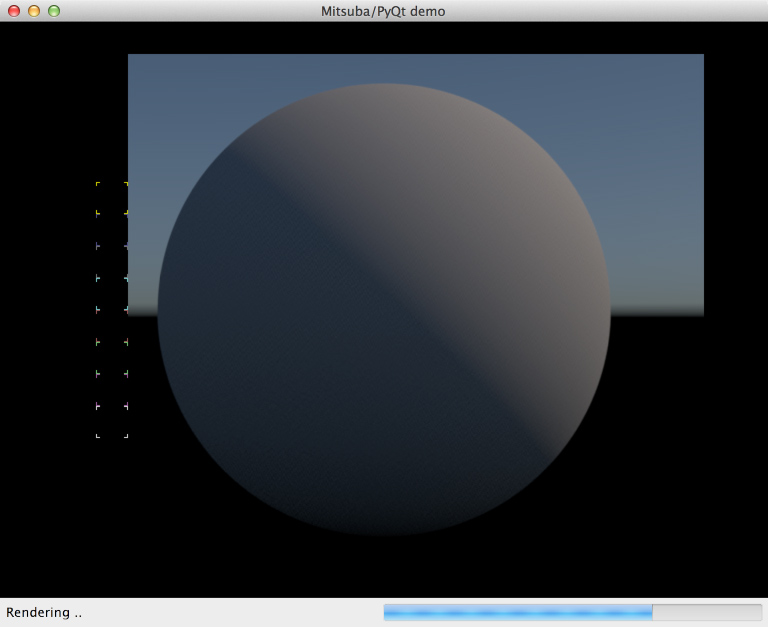
\includegraphics[width=10cm]{images/python_demo.jpg}
\end{center}
When using this snippet, please be wary of threading-related issues; the key thing to remember is that
in Qt, only the main thread is allowed to modify Qt widgets. On the other hand, rendering and logging-related
callbacks will be invoked from different Mitsuba-internal threads---this means that it's not possible to e.g.
directly update the status bar message from the callback \code{finishJobEvent}. To do this, we must use
use Qt's \code{QueuedConnection} to communicate this event to the main thread via signals and slots. See the
code that updates the status and progress bar for more detail.
\begin{python}
import mitsuba, multiprocessing, sys, time

from mitsuba.core import Scheduler, PluginManager, Thread, Vector, Point2i, \
    Vector2i, LocalWorker, Properties, Bitmap, Spectrum, Appender, EWarn, \
    Transform, FileStream
from mitsuba.render import RenderQueue, RenderJob, Scene, RenderListener
from PyQt4.QtCore import Qt, QPoint, QSize, QRect, pyqtSignal
from PyQt4.QtGui import QApplication, QMainWindow, QPainter, QImage, \
    QProgressBar, QWidget, QSizePolicy

Signal = pyqtSignal

class MitsubaRenderBuffer(RenderListener):
    """
    Implements the Mitsuba callback interface to capture notifications about
    rendering progress. Partially completed image blocks are efficiently
    tonemapped into a local 8-bit Mitsuba Bitmap instance and exposed as a QImage.
    """
    RENDERING_FINISHED  = 0
    RENDERING_CANCELLED = 1
    RENDERING_UPDATED   = 2
    GEOMETRY_CHANGED    = 3

    def __init__(self, queue, callback):
        super(MitsubaRenderBuffer, self).__init__()
        self.bitmap = self.qimage = None
        self.callback = callback
        self.time = 0
        self.size = Vector2i(0, 0)
        queue.registerListener(self)

    def workBeginEvent(self, job, wu, thr):
        """ Callback: a worker thread started rendering an image block.
            Draw a rectangle to highlight this """
        _ = self._get_film_ensure_initialized(job)
        self.bitmap.drawWorkUnit(wu.getOffset(), wu.getSize(), thr)
        self._potentially_send_update()

    def workEndEvent(self, job, wr, cancelled):
        """ Callback: a worker thread finished rendering an image block.
            Tonemap the associated pixels and store them in 'self.bitmap' """
        film = self._get_film_ensure_initialized(job)
        film.develop(wr.getOffset(), wr.getSize(), wr.getOffset(), self.bitmap)
        self._potentially_send_update()

    def refreshEvent(self, job):
        """ Callback: the entire image changed (some rendering techniques
            do this occasionally). Hence, tonemap the full film. """
        film = self._get_film_ensure_initialized(job)
        film.develop(Point2i(0), self.size, Point2i(0), self.bitmap)
        self._potentially_send_update()

    def finishJobEvent(self, job, cancelled):
        """ Callback: the rendering job has finished or was cancelled.
            Re-develop the image once more for the final result. """
        film = self._get_film_ensure_initialized(job)
        film.develop(Point2i(0), self.size, Point2i(0), self.bitmap)
        self.callback(MitsubaRenderBuffer.RENDERING_CANCELLED if cancelled
                      else MitsubaRenderBuffer.RENDERING_FINISHED)

    def _get_film_ensure_initialized(self, job):
        """ Ensure that all internal data structure are set up to deal
            with the given rendering job """
        film = job.getScene().getFilm()
        size = film.getSize()

        if self.size != size:
            self.size = size

            # Round the buffer size to the next power of 4 to ensure 32-bit
            # aligned scanlines in the underlying buffer. This is needed so
            # that QtGui.QImage and mitsuba.Bitmap have exactly the same
            # in-memory representation.
            bufsize = Vector2i((size.x + 3) // 4 * 4, (size.y + 3) // 4 * 4)

            # Create an 8-bit Mitsuba bitmap that will store tonemapped pixels
            self.bitmap = Bitmap(Bitmap.ERGB, Bitmap.EUInt8, bufsize)
            self.bitmap.clear()

            # Create a QImage that is backed by the Mitsuba Bitmap instance
            # (i.e. without doing unnecessary bitmap copy operations)
            self.qimage = QImage(self.bitmap.getNativeBuffer(), self.size.x,
                                 self.size.y, QImage.Format_RGB888)

            self.callback(MitsubaRenderBuffer.GEOMETRY_CHANGED)
        return film

    def _potentially_send_update(self):
        """ Send an update request to any attached widgets, but not too often """
        now = time.time()
        if now - self.time > .25:
            self.time = now
            self.callback(MitsubaRenderBuffer.RENDERING_UPDATED)

class RenderWidget(QWidget):
    """ This simple widget attaches itself to a Mitsuba RenderQueue instance
        and displays the progress of everything that's being rendered """
    renderingUpdated = Signal(int)

    def __init__(self, parent, queue, default_size = Vector2i(0, 0)):
        QWidget.__init__(self, parent)
        self.buffer = MitsubaRenderBuffer(queue, self.renderingUpdated.emit)
        # Need a queued conn. to avoid threading issues between Qt and Mitsuba
        self.renderingUpdated.connect(self._handle_update, Qt.QueuedConnection)
        self.setSizePolicy(QSizePolicy.Minimum, QSizePolicy.Minimum)
        self.default_size = default_size

    def sizeHint(self):
        size = self.buffer.size if not self.buffer.size.isZero() else self.default_size
        return QSize(size.x, size.y)

    def _handle_update(self, event):
        image = self.buffer.qimage
        # Detect when an image of different resolution is being rendered
        if image.width() > self.width() or image.height() > self.height():
            self.updateGeometry()
        self.repaint()

    def paintEvent(self, event):
        """ When there is more space then necessary, display the image centered
            on a black background, surrounded by a light gray border """
        QWidget.paintEvent(self, event)
        qp = QPainter(self)
        qp.fillRect(self.rect(), Qt.black)

        image = self.buffer.qimage
        if image is not None:
            offset = QPoint((self.width() - image.width()) / 2,
                (self.height() - image.height()) / 2)
            qp.setPen(Qt.lightGray)
            qp.drawRect(QRect(offset - QPoint(1, 1), image.size() + QSize(1, 1)))
            qp.drawImage(offset, image)
        qp.end()

class MitsubaDemo(QMainWindow):
    renderProgress = Signal(int)

    def __init__(self):
        super(MitsubaDemo, self).__init__()

        # Initialize Mitsuba
        self.initializeMitsuba()
        self.job = self.createRenderJob()
        self.job.setInteractive(True)

        # Initialize the user interface
        status = self.statusBar()
        self.rwidget = RenderWidget(self, self.queue,
            self.scene.getFilm().getSize())
        progress = QProgressBar(status)
        status.setContentsMargins(0,0,5,0)
        status.addPermanentWidget(progress)
        status.setSizeGripEnabled(False)
        self.setWindowTitle('Mitsuba/PyQt demo')
        self.setCentralWidget(self.rwidget)

        # Hide the scroll bar once the rendering is done
        def renderingUpdated(event):
            if event == MitsubaRenderBuffer.RENDERING_FINISHED:
                status.showMessage("Done.")
                progress.hide()

        self.renderProgress.connect(progress.setValue, Qt.QueuedConnection)
        self.rwidget.renderingUpdated.connect(renderingUpdated,
            Qt.QueuedConnection)

        # Start the rendering process
        status.showMessage("Rendering ..")
        self.job.start()

    def initializeMitsuba(self):
        # Start up the scheduling system with one worker per local core
        self.scheduler = Scheduler.getInstance()
        for i in range(0, multiprocessing.cpu_count()):
            self.scheduler.registerWorker(LocalWorker(i, 'wrk%i' % i))
        self.scheduler.start()
        # Create a queue for tracking render jobs
        self.queue = RenderQueue()
        # Get a reference to the plugin manager
        self.pmgr = PluginManager.getInstance()

        # Process Mitsuba log and progress messages within Python
        class CustomAppender(Appender):
            def append(self2, logLevel, message):
                print(message)
            def logProgress(self2, progress, name, formatted, eta):
                # Asynchronously notify the main thread
                self.renderProgress.emit(progress)

        logger = Thread.getThread().getLogger()
        logger.setLogLevel(EWarn) # Display warning & error messages
        logger.clearAppenders()
        logger.addAppender(CustomAppender())

    def closeEvent(self, e):
        self.job.cancel()
        self.queue.join()
        self.scheduler.stop()

    def createRenderJob(self):
        self.scene = self.pmgr.create({
            'type' : 'scene',
            'sphere' : {
                'type' : 'sphere',
            },
            'envmap' : {
                'type' : 'sunsky'
            },
            'sensor' : {
                'type' : 'perspective',
                'toWorld' : Transform.translate(Vector(0, 0, -5)),
                'sampler' : {
                    'type' : 'halton',
                    'sampleCount' : 64
                }
            }
        })

        return RenderJob('rjob', self.scene, self.queue)

    def keyPressEvent(self, e):
        if e.key() == Qt.Key_Escape:
            self.close()

def main():
    import signal
    # Stop the program upon Ctrl-C (SIGINT)
    signal.signal(signal.SIGINT, signal.SIG_DFL)

    app = QApplication(sys.argv)
    demo = MitsubaDemo()
    demo.show()
    demo.raise_()
    retval = app.exec_()
    sys.exit(retval)

if __name__ == '__main__':
    main()
\end{python}


\subsubsection{Mitsuba interaction with NumPy}
Suppose that \code{bitmap} contains a \code{mitsuba.core.Bitmap} instance (e.g. a rendering). Then the following snippet efficiently turns the image into a NumPy array:
\begin{python}
import numpy as np
array = np.array(bitmap.getNativeBuffer())
\end{python}
